\documentclass[a4paper,12pt]{article}
\usepackage{xeCJK}
\usepackage{indentfirst}
\usepackage{amsmath}
\usepackage{amsfonts}
\usepackage{float}
\usepackage{enumerate}
\usepackage{svg}
\usepackage{graphicx}
\usepackage{booktabs}
\usepackage[style=gb7714-2015ay, backend=biber]{biblatex}
\addbibresource{fuck.bib}
\usepackage[hidelinks]{hyperref}
\setcounter{secnumdepth}{0}
\title{Impact of climate change on insurance demand}
\author{董晨阳\and 李昭伦}
\date{\today}
\begin{document}
\maketitle
\tableofcontents
\clearpage
\section{Introduction: impacts on life and non-life insurance might be different}
Climate change can increase losses to property, cause costly disruptions to society, and reduce the affordability of insurance. The frequency and intensity of extreme weather events such as heat waves, droughts, and floods can increase losses to property and cause costly disruptions to society. This can reduce the affordability of insurance. According to McKinsey, demand for insurance will grow in line with investment in technologies that support derisking along the value chain, from manufacturing to deployment to production. While the impact of climate change and the net effect on insurance demand is uncertain, new opportunities will emerge for insurance to support derisking along the value chain.

However, when we talk about the impact of climate change on insurance demand, we can see some differences between life and non-life insurance. Life insurance demand may increase due to the potential health effects of climate change, such as increased mortality and morbidity from heat stress, respiratory diseases, infectious diseases, etc. Non-life insurance demand may also increase due to the physical and transition risks of climate change, such as increased damage to property and infrastructure from extreme weather events, sea level rise, wildfires, etc., as well as increased liability claims from climate-related litigation, regulation, or consumer pressure. But non-life insurance demand may also decrease in some areas where insurance becomes unaffordable or unavailable due to the high frequency or severity of climate-related losses. This can create protection gaps and market failures, especially for vulnerable communities and regions. Therefore we would split our literature review into life and non-life insurance.


\section{The impact of climate on life insurance}
\subsection{Overall effects: climate change increases demand of life insurance}
Generally, climate change would cause more insure incidents and increase risk adverse. Therefore climate change may increase the demand of life insurance. For the overall impact on life insurance, \cite{peara1999global} examines the impact of global climate change on life insurance demand. The author argues that global climate change has significant implications for the life insurance industry as it affects mortality rates, morbidity rates, and the demand for life insurance products. The author also discusses how climate change can affect health organizations by increasing the incidence of certain diseases. The empirical results of this paper suggest that there is a positive relationship between global climate change and life insurance demand. The author finds that there is a significant increase in life insurance demand in areas where there is a high incidence of natural disasters.

\cite{peara1999global} provides valuable insights into the impact of global climate change on the life insurance industry. The author provides a theoretical model that can be used to examine the relationship between global climate change and life insurance demand. The empirical results of this paper suggest that there is a positive relationship between global climate change and life insurance demand. However, it is important to note that this paper was published in 1999 and may not reflect current trends in the industry.

\subsection{Particular Countries empirical results}
For specified countries like the European Union , \cite{melnychenko2021influence} studies the impact of climate change on the life insurance market using panel data from 28 countries of EU for the last 9 years. The study is based on a panel model as follows:
$$Premiums_{i,t}=\beta_0+\beta_1 GGE_{i,t}+\epsilon_{i,t}$$
where the amount of premiums under life insurance contracts is defined as a function of the fundamental factor of climate change(Green-house Gas Emissions).

The authors found that climate change has a significant impact on the life insurance market in the EU. Specifically, they found that climate change has a positive impact on life insurance demand. This means that as climate change continues to affect our planet, it will lead to an increase in demand for life insurance products.

The panel model used in this study is based on a fixed-effects regression model. The authors used this model to estimate the impact of climate change on the life insurance market in the EU. The model includes several control variables such as GDP per capita, population density, and unemployment rate.

The empirical results of \cite{melnychenko2021influence} show that climate change has a significant impact on the life insurance market in the EU. The authors found that an increase in temperature leads to an increase in premiums under life insurance contracts. This means that as climate change continues to affect our planet, it will have an increasingly significant impact on the life insurance market.

In terms of evaluating this article’s value, it provides valuable insights into the impact of climate change on the life insurance market in the EU. The authors used a fixed-effects regression model to estimate this impact and evaluated their results by comparing them with previous studies. However, it is important to note that this study only focuses on the EU and may not be applicable to other regions or countries.

\cite{ford2019practical} notes that climate change could have a significant impact on life insurance demand in UK. For example, changes in temperature and precipitation patterns could lead to an increase in the incidence of certain diseases, which could in turn increase mortality rates. The guide also notes that climate change could lead to changes in consumer behavior, such as a shift towards more sustainable products and services.

In terms of the value of this article, it is important to note that this guide was produced by the Sustainability Board of the Institute and Faculty of Actuaries in the UK. The IFoA is a professional body for actuaries in the UK and internationally. The guide is part of a series of practical guides that the Sustainability Board has produced/is producing. Other practical guides in this series include: DB Pensions (with accompanying papers around mortality and covenants), DC Pensions, and Practical Guide to Climate Change for General Insurance Actuaries.
\begin{figure}[H]
    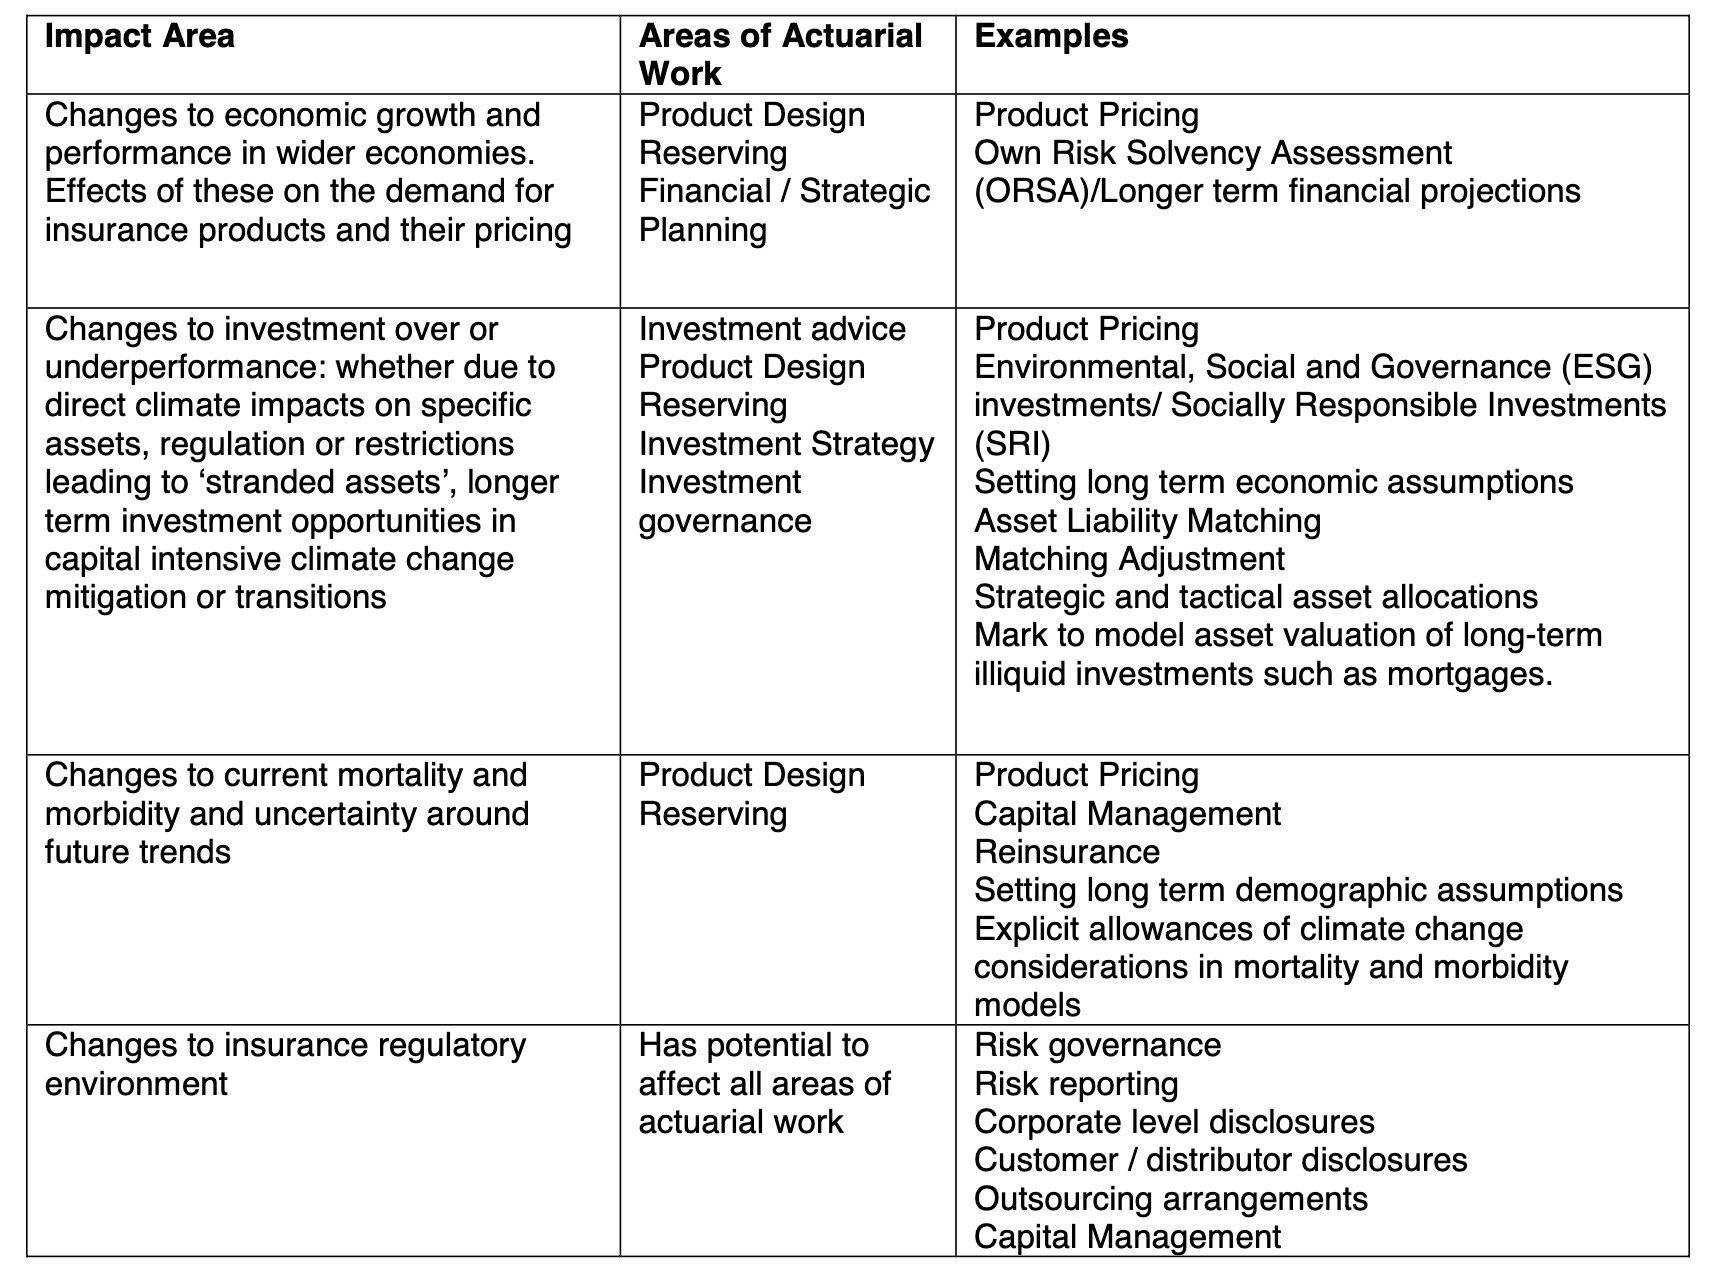
\includegraphics[width=\linewidth]{img/actuarial.png}
    \caption{Possible impacts on actuaries}
\end{figure}

\cite{medders2017climate} examines the impact of climate change on insurance in Florida. It argues that climate change has significant positive impacts on the insurance industry in Florida. The author notes that Florida is particularly vulnerable to climate change due to its location and geography. It examines the impact of climate change on life insurance demand, and finds that there is a significant increase in demand for life insurance as a result of climate change. Model used in the paper is based on a regression analysis of data from the National Flood Insurance Program (NFIP) and the National Oceanic and Atmospheric Administration (NOAA). The empirical results show that there is a significant increase in demand for life insurance as a result of climate change. The paper concludes that the impact of climate change on insurance in Florida is significant and that it is important for insurers to take this into account when setting premiums.

\subsection{How life insurers react to climate change and increasing demand}
\cite{gupta2023assessing} aims to assess and distinguish between insurance firms by impact and response to climate change and relate the firms’ financial characteristics to climate risk exposure. The paper uses a text mining approach using climate change sub-dictionaries on risk exposure, impact, and response, and a nested feature extraction method is developed to define and classify. The paper argues that climate change poses a serious risk for insurance firms, threatening their sustainability from numerous channels of impact. The paper also argues that life insurance demand is expected to increase due to climate change. The empirical result also shows that the insurance industry has been responding to climate risks by increasing their investment in renewable energy sources.

\cite{miljkovic2018examining} analyzes the impact on overall mortality rates for the general US population arising from climate change and the weather events resulting in property damages for the period 1968–2013. The authors develop a fixed effects panel data model for the impact of climate change on property damage, with precipitation having a more pronounced effect than extreme temperatures.

The paper argues that climate change has a significant impact on life insurance demand. The authors suggest that life insurance companies should consider the impact of climate change on mortality rates when pricing their policies. They also suggest that life insurance companies should consider offering policies that are specifically designed to protect against the risks associated with climate change.

The model used in this paper is a fixed effects panel data model. This model is used to estimate the impact of climate change on property damage and overall mortality rates. The authors use data from 1968 to 2013 to estimate the model. The empirical results of this paper suggest that climate change has a significant impact on overall mortality rates. The authors find that precipitation has a more pronounced effect on mortality rates than extreme temperatures. They also find that the impact of climate change on mortality rates is more pronounced in urban areas than in rural areas.

\section{The impact of climate on non-life insurance}
These papers investigate the impact of climate change on non-life insurance demand, focusing on flood insurance, index insurance, and crop insurance. The studies explore the role of insurance as a financial instrument to manage climate-related risks, the determinants of insurance demand, and the welfare effects of insurance under different climate change scenarios.

The literature reveals that climate change exacerbates risks associated with extreme weather events, influencing the demand for various types of insurance. Factors such as income level, risk aversion, risk perception, and policy design significantly impact insurance demand and supply. Furthermore, basis risk is identified as a critical factor affecting the functioning and demand for index insurance.

Several studies find that insurance provides modest welfare gains for policyholders, but it may also reduce their incentives to adopt other adaptation measures. The impact of climate change on insurance demand varies across regions and countries, with both positive and negative effects observed depending on the balance between risk exposure and risk reduction.

The papers propose policy recommendations to improve the design and implementation of insurance schemes, such as reducing basis risk, increasing premium differentiation, promoting complementary adaptation measures, and enhancing policyholders' awareness and education. These measures can help enhance the role of insurance as a strategy for adapting to climate change and managing its associated risks.
\subsection{Overall impact on non-life insurance}
Clement et al. (2018) review the literature on the problem of basis risk in index insurance, which occurs when insurance payouts depend on an index imperfectly related to actual losses experienced by the policyholder. They identify four main themes in the literature, including index design, data quality and sampling, basis risk estimation, and insurance demand and supply. They offer policy recommendations to reduce basis risk and enhance the uptake of index insurance as a climate change adaptation strategy.

Clement et al. (2018) reviews the literature on the problem of basis risk in index insurance, which occurs when insurance payouts depend on an index that is imperfectly related with actual losses experienced by the policyholder. The paper focuses on the design of the index, the quality and sampling of data, the estimation of basis risk and its influence on insurance demand, and the supply of index insurance. The paper also provides policy recommendations to reduce basis risk and enhance the uptake of index insurance as a climate change adaptation strategy.

The paper acknowledges that climate change is increasing the risks of weather-related disasters in many regions around the world, which has an adverse socio-economic impact on households, farmers and small businesses. The paper argues that index insurance can be a useful instrument to manage climate risks and enhance financial resilience, especially in low-income countries where traditional insurance is often unavailable or unaffordable. However, the paper also recognizes that index insurance faces several challenges, such as low demand, high transaction costs, and limited supply. The paper claims that basis risk is one of the main factors that affect the functioning and demand for index insurance, as it reduces the expected benefits and increases the uncertainty of insurance coverage.

Clement et al. (2018) uses a narrative review method to synthesize the existing literature on basis risk in index insurance. They identifies four main themes in the literature: (i) index design, which involves choosing the type and level of aggregation of the index, selecting the appropriate weather or biophysical parameters, and defining the trigger and payout functions; (ii) data quality and sampling, which refers to the availability and accuracy of historical and real-time data on weather variables and crop yields, as well as the spatial and temporal resolution of data collection; (iii) basis risk estimation, which involves measuring the degree of correlation between the index and actual losses, as well as assessing the distributional impacts of basis risk across different groups of policyholders; and (iv) insurance demand and supply, which examines how basis risk affects the willingness to pay for and purchase index insurance, as well as how it influences the profitability and sustainability of index insurance providers.

The authors finds that basis risk is a pervasive and complex problem in index insurance that depends on various factors, such as weather variability, crop heterogeneity, data availability, index design choices, and policyholder characteristics. The paper reports that most studies show that index insurance participation is higher when basis risk is low, but only a few studies analyze how the magnitude of basis risk influences demand by using actual household level data. The paper also finds that basis risk can have negative impacts on both policyholders and insurers, such as reducing welfare gains, discouraging investment in productive activities, eroding trust in insurance providers, increasing moral hazard and adverse selection problems, and lowering market penetration rates.

The paper contributes to the literature on index insurance by providing a comprehensive and systematic review of the impact of basis risk on the functioning of and demand for index insurance. The paper also offers policy implications for reducing basis risk and enhancing the uptake of index insurance as a climate change adaptation strategy. Some of these implications include: improving data quality and availability; involving stakeholders in index design; combining index insurance with other risk management tools; providing subsidies or premium discounts; increasing financial literacy and awareness; creating public-private partnerships; and establishing regulatory frameworks and consumer protection mechanisms

Following that, Ranger and Surminski (2013) examine how climate change may influence non-life insurance demand trends in "the BRICS" up to 2030. They project the growth of gross premium volumes in these countries under different scenarios of income and insurance penetration. Their findings suggest that climate change may have both positive and negative impacts on insurance demand, but these impacts are likely to be small relative to income effects.

The paper examines how climate change may influence the trends and drivers of non-life insurance demand in the BRICS in the period to 2030. The paper uses a simple model to project the growth of gross premium volumes in these countries under different scenarios of income and insurance penetration. The paper also identifies five pathways through which climate change may affect insurance demand: wealth; willingness to pay; policy and regulation; supply of insurance; and new opportunities related to adaptation and mitigation.

The authors assumes that climate change will increase the frequency and intensity of extreme weather events that can cause losses to property and assets. The paper argues that climate change can have both positive and negative impacts on insurance demand, depending on the balance between risk exposure and risk reduction. The paper hypothesizes that, with the exception of policy and regulation, the influence of climate change on insurance demand to 2030 is likely to be small when compared with the expected growth due to rising incomes, but is not insignificant. The paper also suggests that the scale and direction of the impacts will depend partly on the responses of insurers and policyholders to the challenges of climate change.

The paper uses a two-step approach to model non-life insurance demand in the BRICS. In the first step, the paper estimates a panel data regression model to identify the determinants of insurance penetration across 40 countries over the period 1996-2010. The paper finds that income per capita, urbanization, financial development, institutional quality, and disaster risk are significant factors that explain cross-country variation in insurance penetration. In the second step, the paper uses the estimated coefficients from the regression model to project gross premium volumes in the BRICS under different scenarios of income growth and insurance penetration. The paper also uses a literature review method to assess the potential impacts of climate change on insurance demand through the five pathways mentioned above.

Ranger and Surminski (2013) finds that non-life insurance demand in the BRICS is expected to grow significantly over the next two decades, driven mainly by rising incomes and increasing insurance penetration. The paper projects that gross premium volumes in these countries could increase at a rate of between 5.4 and 12.3 percent per year over the coming decade, depending on the country and scenario. The paper also finds that climate change may have both positive and negative impacts on insurance demand through various pathways, but these impacts are likely to be small relative to income effects. For example, the paper estimates that climate change may reduce premium growth by less than 0.4 percentage points per year through its impact on wealth. However, the paper also acknowledges that there are large uncertainties and data gaps that limit the robustness of these estimates.

The paper contributes to the literature on non-life insurance demand in emerging economies by providing a comprehensive analysis of the potential impacts of climate change on this sector. The paper also provides policy implications for enhancing the role of insurance as a strategy for adapting to climate change, such as improving data quality and availability; reducing basis risk and transaction costs; increasing financial literacy and awareness; creating public-private partnerships; and establishing regulatory frameworks and consumer protection mechanisms.

\subsection{Impact on specified non-life insurance: crop and flood insurance}

Firstly, Tesselaar et al. (2020) examine the potential socio-economic tipping-point in Europe for current flood insurance systems under different scenarios of climate and socio-economic change. They use the Dynamic Integrated Flood and Insurance (DIFI) model to simulate the impacts of various scenarios on flood insurance premiums and consumer demand. The paper finds that regional inequalities in flood insurance affordability and uptake are exacerbated by climate change.

The paper examines whether a socio-economic tipping-point can occur in Europe for current flood insurance systems under different scenarios of climate and socio-economic change. A tipping-point is defined as a situation where the demand for flood insurance almost disappears due to rising unaffordability and declining willingness to purchase coverage. The paper also analyzes regional inequalities in the ability to use flood insurance as an adaptation instrument to changing flood risk.

They assume that climate change will increase flood risk and cause higher risk-based insurance premiums in the future. The paper argues that this will reduce the demand for flood insurance, especially among low-income households who may not be able to afford coverage or who may have fatalistic beliefs about the consequences of climate change. The paper hypothesizes that a tipping-point can occur in some regions under a high climate change scenario, where the functioning of a formal flood insurance system is hampered by diminishing demand for coverage.

They use the “Dynamic Integrated Flood and Insurance” (DIFI) model to simulate the impacts of various scenarios of climate and socio-economic change on flood insurance premiums and consumer demand. The DIFI model integrates flood risk simulations from the LISFLOOD model with a discrete choice experiment that elicits farmers’ preferences for two types of insurance plans: standard and index-based. The DIFI model also incorporates income distribution data and income elasticity of insurance demand to estimate the affordability and uptake of flood insurance across regions.

They find that unaffordability and declining demand for flood insurance increase across scenarios towards 2080. Under a high climate change scenario, the paper shows that a tipping-point occurs in several regions, such as Southern Europe, Eastern Europe, and parts of Western Europe, where insurance uptake drops below 10\%. The paper also finds that regional inequalities in flood insurance affordability and uptake are exacerbated by climate change, as some regions face higher flood risk and lower income levels than others.

The paper contributes to the literature on flood insurance demand in Europe by exploring the possibility of a socio-economic tipping-point under climate change and by highlighting regional inequalities in flood insurance affordability and uptake. The paper also provides policy implications for the design and reform of flood insurance arrangements, such as introducing subsidies, caps, or public-private partnerships to enhance the accessibility and attractiveness of flood insurance for low-income households and high-risk regions.

Subsequently, Botzen and Van den Bergh (2012) investigate the demand for flood insurance by Dutch homeowners under different scenarios of climate change and government compensation. They find a positive but moderate demand for flood insurance among Dutch homeowners and show that flood insurance demand is influenced by both climatic and non-climatic factors. They also find that flood insurance reduces homeowners’ perceived flood risk and their incentives to invest in flood-proofing measures.

The paper investigates the demand for flood insurance by Dutch homeowners under different scenarios of climate change and government compensation. The paper uses a stated preference survey with a choice experiment to elicit the willingness to pay (WTP) for flood insurance with various attributes, such as premium rate, coverage level, deductible, and payout delay. The paper also estimates the welfare effects of flood insurance and its impact on risk perception and risk reduction behavior.

The paper assumes that climate change will increase the frequency and intensity of flood events in the Netherlands, which poses a significant risk to property and assets. The paper argues that flood insurance can be a valuable instrument to reduce the financial vulnerability of homeowners and to enhance their adaptation capacity. However, the paper also recognizes that flood insurance faces several challenges, such as moral hazard, adverse selection, basis risk, and crowding out of other risk management measures. The paper hypothesizes that flood insurance demand depends on various factors, such as income level, risk aversion, risk perception, flood experience, and policy design.

The paper uses a mixed logit model to analyze the data from a choice experiment conducted with 1,000 Dutch homeowners in 2008. The choice experiment presented respondents with two hypothetical flood insurance plans with different attributes and asked them to choose one plan or none. The paper also used a simulation method to calculate the expected utility gain from flood insurance and its impact on risk perception and risk reduction behavior. The paper used secondary data on flood risk and damage scenarios to calibrate the choice experiment and the simulation model.

The paper finds that there is a positive but moderate demand for flood insurance among Dutch homeowners, with an average WTP of €98 per year for a standard insurance plan. The paper shows that flood insurance demand is influenced by both climatic and non-climatic factors. The paper finds that climate change scenarios have a positive but small effect on WTP, while government compensation scenarios have a negative but large effect on WTP. The paper also finds that flood insurance provides a positive but modest welfare gain for homeowners, equivalent to 0.5 percent of their expected income. However, the paper also finds that flood insurance reduces homeowners’ perceived flood risk and their incentives to invest in flood-proofing measures.

The paper contributes to the literature on flood insurance and climate change adaptation by providing empirical evidence on the determinants and welfare effects of flood insurance in a European context where no private insurance is currently available. The paper also provides policy implications for improving the design and implementation of flood insurance schemes, such as reducing basis risk, increasing premium differentiation, promoting complementary adaptation measures, and enhancing homeowners’ awareness and education.

Besides flood insurance, Akter et al. (2017) investigate how climate change skepticism, farmers’ fatalistic beliefs, and insurance plan design influence farmers’ interest in crop weather insurance in coastal Bangladesh. The paper uses a discrete choice experiment to elicit farmers’ preferences for index versus standard insurance options for maize production. The paper also examines the relationship between farmers’ concern about the adverse livelihood impacts of climate change and their demand for insurance.

The paper argues that climate change skepticism and fatalism are important barriers to farmers’ adoption of crop insurance as a climate change adaptation strategy. The paper hypothesizes that farmers who are more concerned about the negative effects of climate change on their livelihoods are more likely to demand insurance, while farmers who exhibit fatalistic views regarding the consequences of climate change are less likely to opt for insurance. The paper also expects that farmers prefer standard insurance over index-based insurance, as the former provides more certainty and transparency in damage compensation.

They uses a multinomial logit model to analyze the data from a discrete choice experiment conducted with 300 maize farmers on a climate-risk prone island in coastal Bangladesh. The choice experiment presented farmers with two hypothetical insurance plans: a standard plan that compensates farmers based on post-hazard assessment of crop damage, and an index plan that compensates farmers based on a set of weather parameter thresholds. The choice experiment also varied the attributes of the insurance plans, such as premium rate, coverage level, payout frequency, and payout delay.

They finds that most farmers were insurance averse, and only 28\% of them chose either standard or index-based insurance over no insurance. Among those who chose insurance, 85\% preferred standard insurance over index-based insurance. The paper also finds that farmers’ concern about the adverse livelihood impacts of climate change was positively and significantly correlated with their demand for insurance, while fatalism was negatively and significantly correlated with their demand for insurance. Other factors that influenced farmers’ insurance demand were farm size, education level, income level, and previous experience with natural disasters.

The paper contributes to the literature on crop insurance demand in developing countries by highlighting the role of climate change skepticism and fatalism as psychological barriers to adaptation. The paper also provides empirical evidence on farmers’ preferences for standard versus index-based insurance plans, which has implications for the design and implementation of crop weather insurance schemes. The paper suggests that policy interventions should aim to increase farmers’ awareness and understanding of climate change risks and the benefits of adaptation, as well as to improve the trustworthiness and accessibility of insurance providers.

Di Falco et al. (2014) explore the role of crop insurance as a financial instrument to hedge against climate change implications using a unique panel dataset of Italian farms. They find that crop insurance demand and supply are influenced by both climatic and non-climatic factors and that crop insurance provides a positive but modest welfare gain for farmers. However, they also find that crop insurance reduces farmers’ incentives to adopt other adaptation measures.

The paper explores the role of crop insurance as a financial instrument to hedge against the implications of climate change. The paper uses a comprehensive estimation strategy and a unique panel dataset to study the determinants of crop insurance demand and supply in Italy, where crop insurance is subsidized by the government. The paper also analyzes the welfare effects of crop insurance and its impact on farmers’ adaptation decisions.

Di Falco et al. (2014) assumes that climate change will increase the frequency and intensity of extreme weather events that can cause crop losses. The paper argues that crop insurance can be a useful tool to reduce farmers’ exposure to climate risk and to enhance their financial resilience. However, the paper also recognizes that crop insurance faces several challenges, such as moral hazard, adverse selection, basis risk, and crowding out of other adaptation measures. The paper hypothesizes that crop insurance demand and supply depend on various factors, such as weather variability, crop characteristics, income level, risk aversion, and policy design.

The authors uses a two-stage estimation approach to model crop insurance demand and supply. In the first stage, the paper estimates a probit model to identify the factors that influence farmers’ decision to purchase crop insurance. In the second stage, the paper estimates a censored regression model to determine the factors that affect the amount of insurance coverage purchased by farmers. The paper also uses a simulation method to calculate the expected utility gain from crop insurance and its impact on farmers’ adaptation behavior. The paper uses a panel dataset of 16,000 Italian farms over the period 2003-2010, which contains information on farm characteristics, crop production, weather conditions, and insurance contracts.

The paper finds that crop insurance demand and supply are influenced by both climatic and non-climatic factors. The paper shows that weather variability, crop type, farm size, income level, risk aversion, and policy design are significant determinants of crop insurance demand and supply. The paper also finds that crop insurance provides a positive but modest welfare gain for farmers, equivalent to 1.5 percent of their expected income. However, the paper also finds that crop insurance reduces farmers’ incentives to adopt other adaptation measures, such as irrigation or diversification.

Di Falco et al. (2014) contributes to the literature on crop insurance and climate change adaptation by providing empirical evidence on the determinants and welfare effects of crop insurance in a European context. The paper also provides policy implications for improving the design and implementation of crop insurance schemes, such as reducing basis risk, increasing premium differentiation, promoting complementary adaptation measures, and enhancing farmers’ awareness and education.

\section{Conclusion: there are opportunities for insurers}

Climate change is a major challenge for the insurance industry, as it affects both the demand and supply of insurance products and services. However, climate change can create new opportunities for insurers to provide solutions for the net-zero transition, such as insuring renewable energy projects, electric vehicles, and carbon capture technologies. It can also increase the demand for risk transfer solutions for rising physical risks, such as extreme weather events, sea level rise, and biodiversity loss. However, climate change can also pose significant threats to insurers, as it can increase the frequency and severity of natural disasters, reduce the affordability and availability of insurance, and expose insurers to regulatory and reputational risks. Therefore, insurers need to adapt their business models and strategies to address the impacts of climate change and support a low-carbon economy. Some of the opportunities for insurers may be:
\begin{enumerate}
    \item Developing new and innovative products and services that address the emerging needs and preferences of customers, such as renewable energy insurance, climate litigation insurance, parametric insurance, etc.
    \item Providing adaptation and resilience services that help customers reduce their exposure and vulnerability to climate risks, such as risk assessments, loss prevention, risk mitigation, etc.
    \item Investing in low-carbon and climate-resilient assets that support the transition to a net-zero economy and generate long-term returns, such as green bonds, renewable energy projects, carbon capture and storage technologies, etc.
    \item Leveraging their expertise and influence to advocate for climate action and awareness among stakeholders, such as regulators, policymakers, investors, consumers, etc.
\end{enumerate}
\nocite{*}
\appendix
\printbibliography
\end{document}
